\section{Variance Floor, Scaling Laws, and Four-Family Generalization (\textbf{RQ1})}
\label{sec:grounding}

\subsection{Four-Level Variance Decomposition Across Six Checkpoints}
\label{sec:variance}

Before attributing localization shifts to surface material conversion, one must establish how much variance stems from inference repeatability, decoding stochasticity, or Monte Carlo path tracing \citep{Zhao2021Calibrate}. On three stratified control scenes (48 paired captures, 96 images), Table~\ref{tab:variance} and Figure~\ref{fig:variance_scaling}(a) decompose four nested variability levels across all six checkpoints:
\begin{enumerate}
    \item \textbf{Level 1 (Greedy process repeat: $0.00\%$, $0.00\,\mathrm{px}$ on all six checkpoints).} Across repeated deterministic inference runs ($T{=}0$, \texttt{do\_sample=False})---three runs on \textsc{Qwen3-VL-8B} and \textsc{Qwen3-VL-32B} (288 pairwise comparisons each) and two runs on \textsc{Qwen3-VL-2B}, \textsc{InternVL3.5-8B-HF}, \textsc{Molmo2-8B}, and \textsc{LLaVA-NeXT-Mistral-7B} (96 comparisons each)---pairwise hit disagreement and spatial coordinate displacement remain strictly zero ($0.00\%$, $0.00\,\mathrm{px}$).
    \item \textbf{Level 2 (Stochastic decoding noise: $8.96\%$ pairwise, $16.67\%$ any-flip).} Repeating the same 96 frozen images across five stochastic draws ($T{=}0.2$, $\text{top-}p{=}0.95$) on \textsc{Qwen3-VL-8B} (960 pairwise checks) produces $94.38\%$ response phrasing variation, $8.96\%$ pairwise hit disagreement, $16.67\%$ of inputs with at least one pass/fail flip, and $16.37\,\mathrm{px}$ mean displacement. This stochastic noise floor explains why stochastic sampling confounds shading studies (\ref{app:archive}) and motivates locking greedy $T{=}0$ decoding to isolate visual sensitivity.
    \item \textbf{Level 3 (Monte Carlo ray-tracing re-render floor).} Holding geometry, cameras, prompts, and \original\ materials fixed across three independent path-tracing renders (96 pairs per model) yields $7.29\%$ ($7/96$, $30.96\,\mathrm{px}$) flips on \textsc{Qwen3-VL-2B}, $5.21\%$ ($5/96$, $24.38\,\mathrm{px}$) on \textsc{LLaVA-NeXT-Mistral-7B}, $3.13\%$ ($3/96$, $9.52\,\mathrm{px}$) on \textsc{Qwen3-VL-8B}, $1.04\%$ ($1/96$) on both \textsc{InternVL3.5-8B-HF} ($10.38\,\mathrm{px}$) and \textsc{Qwen3-VL-32B} ($6.39\,\mathrm{px}$), and $0.00\%$ ($0/96$, $5.98\,\mathrm{px}$) on \textsc{Molmo2-8B}.
    \item \textbf{Level 4 (Material conversion on the same 48 control pairs).} Lowering \textsc{MDL} to \usdps{} induces \textbf{$2.00\times$ to $6.00\times$} the flip rate of independent path-tracing repeats ($20.83\%$ on 2B [$2.86\times$], $10.42\%$ on \textsc{LLaVA-NeXT} [$2.00\times$], $8.33\%$ on 8B [$2.67\times$], $6.25\%$ on \textsc{InternVL3.5-8B} [$6.00\times$], $4.17\%$ on \textsc{32B} [$4.00\times$], and $4.17\%$ vs.\ $0.00\%$ [$>4\times$] on \textsc{Molmo2-8B}), alongside $2.1\times$ to $7.0\times$ larger spatial shifts ($23.26\text{--}65.64\,\mathrm{px}$).
\end{enumerate}

\begin{table*}[!t]
\centering\scriptsize
\resizebox{\textwidth}{!}{% Verified from paper/shared/evidence/raw/cviu_v3/variance_decomposition.json
\begin{tabular*}{\textwidth}{@{\extracolsep{\fill}}llrrrrrr@{}}
\toprule
Model (Strict \texttt{bfloat16}) & Family & L1 Greedy & \multicolumn{2}{c}{L3: Re-Render Floor (96)} & \multicolumn{2}{c}{L4: Conversion (48 pairs)} & L4 / L3 \\
\cmidrule(lr){4-5} \cmidrule(lr){6-7}
 & & Disagr.\ (pairs) & Flip Rate & Shift (px) & Flip Rate & Shift (px) & Ratio \\
\midrule
Qwen3-VL-2B & Qwen3-VL & 0.00\% (96) & 7.29\% (7/96) & 30.96 & \textbf{20.83\%} (10/48) & \textbf{65.64} & 2.86$\times$ \\
LLaVA-NeXT-Mistral-7B & Mistral + CLIP & 0.00\% (96) & 5.21\% (5/96) & 24.38 & \textbf{10.42\%} (5/48) & \textbf{59.90} & 2.00$\times$ \\
InternVL3.5-8B-HF & InternVL3.5 & 0.00\% (96) & 1.04\% (1/96) & 10.38 & \textbf{6.25\%} (3/48) & \textbf{39.23} & 6.00$\times$ \\
Qwen3-VL-8B & Qwen3-VL & 0.00\% (288) & 3.13\% (3/96) & 9.52 & \textbf{8.33\%} (4/48) & \textbf{23.83} & 2.67$\times$ \\
Molmo2-8B & Molmo2 (SigLIP-2) & 0.00\% (96) & 0.00\% (0/96) & 5.98 & \textbf{4.17\%} (2/48) & \textbf{41.64} & $>4\times$ \\
Qwen3-VL-32B & Qwen3-VL & 0.00\% (288) & 1.04\% (1/96) & 6.39 & \textbf{4.17\%} (2/48) & \textbf{23.26} & 4.00$\times$ \\
\midrule
\multicolumn{8}{@{}l}{\emph{Level 2 stochastic decoding baseline (Qwen3-VL-8B, $T{=}0.2$, $\text{top-}p{=}0.95$, 5 draws on same 96 frozen images, 960 pairs):}} \\
\multicolumn{2}{@{}l}{Pairwise hit disagreement / any-flip across 5 draws} & \multicolumn{6}{r@{}}{8.96\% pairwise disagreement (16.67\% inputs with $\ge 1$ flip; 94.38\% text change; 16.37\,px shift)} \\
\bottomrule
\end{tabular*}
}
\caption{Four-level variance decomposition over the three stratified control scenes (48 object pairs, 96 images) across all six checkpoints. Greedy decoding eliminates sampling stochasticity ($0.00\%$ everywhere), establishing material conversion well above the independent ray-tracing noise floor.}
\label{tab:variance}
\end{table*}

\begin{figure*}[!t]
\centering
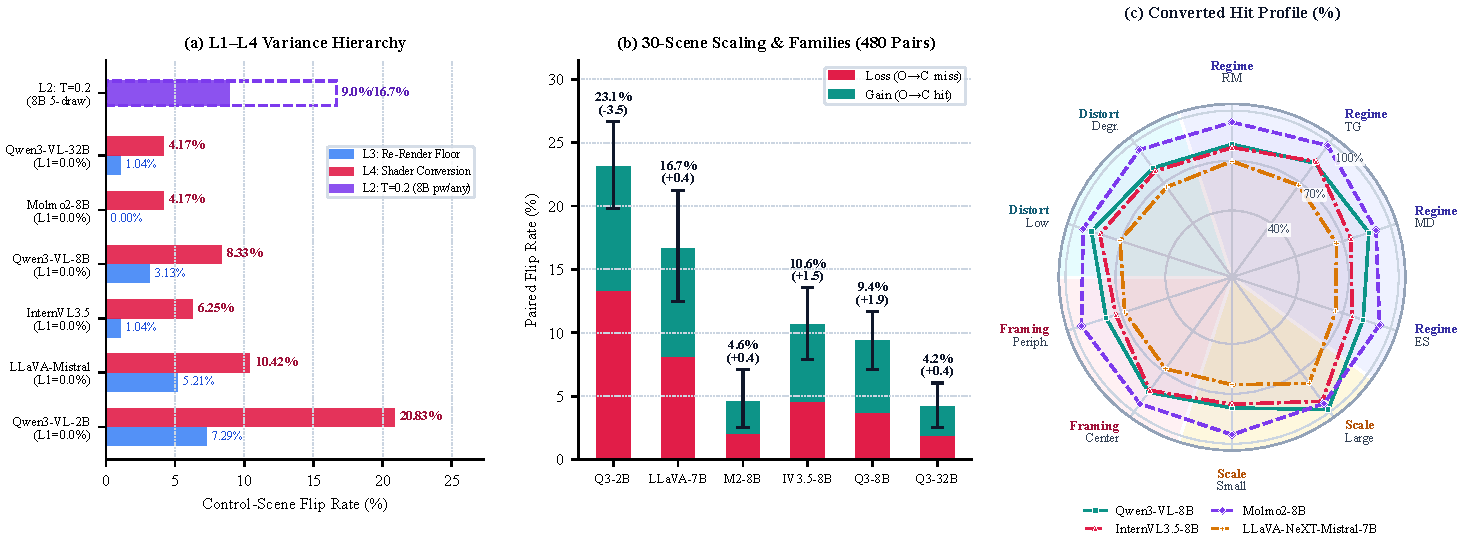
\includegraphics[width=\textwidth]{fig4_variance_and_polar.pdf}
\caption{\textbf{Four-level variance hierarchy, 30-scene scaling across four families, and converted hit profile.}
\emph{(a)} Across all six checkpoints, greedy $T{=}0$ inference eliminates decoding noise ($0.00\%$), while \textsc{MDL} $\to$ \usdps{} conversion (Level 4) induces $2.0\times$ to $6.0\times$ more flips than same-material ray-tracing repeats (Level 3; $4.17\%$ vs.\ $0.00\%$ on \textsc{Molmo2-8B}).
\emph{(b)} Across 30 scenes (480 pairs), scaling \textsc{Qwen3-VL} $16\times$ (2B $\to$ 8B $\to$ 32B) reduces turnover from $23.13\%$ to $4.17\%$, yet bidirectional swaps persist across all four independent families (\textsc{InternVL3.5}, \textsc{Molmo2}, \textsc{LLaVA-NeXT-Mistral}). Error bars denote 10,000-draw scene-cluster 95\% CIs.
\emph{(c)} Multi-axis polar profile of \converted\ hit rate ($H_C$, \%) across residential/commercial domains, optical regimes, and target scales.}
\label{fig:variance_scaling}
\end{figure*}

\subsection{30-Scene Scaling Laws and Four-Family Generalization}
\label{sec:scaling}

Table~\ref{tab:grounding_v3} and Figure~\ref{fig:variance_scaling}(b)--(c) evaluate all six checkpoints across the full 30-scene suite (480 paired captures, $96.5\%\text{--}100.0\%$ valid parse rates). Four empirical patterns characterize how shader lowering affects grounding behavior:

\paragraph{1.\ Near-zero net deltas conceal $4.17\%\text{--}23.13\%$ bidirectional turnover.}
Three checkpoints spanning completely distinct model families record the exact same aggregate delta of $+0.42\%$ between \original\ and \converted: \textsc{LLaVA-NeXT-Mistral-7B} ($67.50\% \to 67.92\%$, 95\% CI $[-3.33\%, +3.96\%]$), \textsc{Qwen3-VL-32B} ($91.67\% \to 92.08\%$, CI $[-1.25\%, +2.29\%]$), and \textsc{Molmo2-8B} ($93.96\% \to 94.38\%$, CI $[-1.67\%, +2.50\%]$). Underneath those nearly flat averages, \textsc{LLaVA-NeXT-Mistral-7B} reverses outcomes on $16.67\%$ of objects ($8.13\%$ Loss, $8.54\%$ Gain; $65.08\,\mathrm{px}$ mean displacement), \textsc{Molmo2-8B} flips $4.58\%$ ($2.08\%$ Loss, $2.50\%$ Gain; $33.80\,\mathrm{px}$), and \textsc{Qwen3-VL-32B} flips $4.17\%$ ($1.88\%$ Loss, $2.29\%$ Gain; $20.78\,\mathrm{px}$). Smaller models exhibit even larger turnover behind modest marginal changes: \textsc{Qwen3-VL-2B} declines $-3.54\%$ net ($66.67\% \to 63.13\%$) while flipping \textbf{$23.13\%$} of pairs ($13.33\%$ Loss, $9.79\%$ Gain; $69.70\,\mathrm{px}$).

\paragraph{2.\ Scaling $16\times$ dampens turnover monotonically yet leaves an irreducible floor}
Within the \textsc{Qwen3-VL} family \citep{Bai2025Qwen3}, scaling from 2B $\to$ 8B $\to$ 32B lifts baseline \original\ accuracy ($66.67\% \to 81.25\% \to 91.67\%$), reduces conditional regression risk $\Pr(H^C{=}0 \mid H^O{=}1)$ roughly tenfold ($20.00\% \to 4.62\% \to 2.05\%$), and lowers overall decision turnover from $23.13\%$ to $9.38\%$ and $4.17\%$ (paired scene-cluster reduction $-18.96$ pp from 2B to 32B, 95\% CI $[-22.92, -15.00]$; $-5.21$ pp from 8B to 32B, CI $[-7.71, -2.71]$). Even at 32B, however, turnover ($4.17\%$) stays $4\times$ above its ray-tracing repeat floor ($1.04\%$) with $20.78\,\mathrm{px}$ average point displacement, while conditional recovery on initially missed objects remains nearly constant around $28\%\text{--}30\%$ across all three scales ($29.38\%$ at 2B, $30.00\%$ at 8B, $27.50\%$ at 32B).

\paragraph{3.\ Cross-family invariance and architecture-specific failures ($85.7\%$ divergence)}
Extending evaluation to three additional VLM families at the 7B--8B scale shows that shader sensitivity generalizes across backbones:
\begin{itemize}
    \item \textsc{InternVL3.5-8B-HF} \citep{Wang2025InternVL35} tracks \textsc{Qwen3-VL-8B} closely in hit rate ($78.54\% \to 80.00\%$, $\Delta H = +1.46\%$) and decision turnover ($10.63\%$; paired difference $+1.25\%$ vs.\ \textsc{Qwen3-VL-8B}, CI $[-2.29\%, +4.79\%]$), though with larger spatial displacements ($47.11\,\mathrm{px}$ vs.\ $27.23\,\mathrm{px}$, paired $+19.88\,\mathrm{px}$).
    \item \textsc{Molmo2-8B} \citep{Clark2026Molmo2}, a \textsc{SigLIP-2} pointing specialist, attains the highest accuracy ($93.96\% \to 94.38\%$) and lowest 8B turnover ($4.58\%$, $-4.79\%$ vs.\ \textsc{Qwen3-VL-8B}, CI $[-7.08\%, -2.50\%]$, with $41.38\%$ conditional recovery), yet its conversion flip rate remains well above its zero ray-tracing noise floor ($4.17\%$ vs.\ $0.00\%$ on controls; $33.80\,\mathrm{px}$ displacement).
    \item \textsc{LLaVA-NeXT-Mistral-7B} \citep{Liu2024LLaVANeXT}, pairing a \textsc{Mistral-7B} language backbone with a \textsc{CLIP} vision encoder, scores $67.50\% \to 67.92\%$ ($\Delta H = +0.42\%$) while incurring $16.67\%$ bidirectional turnover ($+7.29\%$ vs.\ \textsc{Qwen3-VL-8B}, CI $[+3.33\%, +11.67\%]$; $65.08\,\mathrm{px}$ shift).
\end{itemize}
Comparing the four $\ge$7B architectures (\textsc{Qwen3-VL-8B}, \textsc{InternVL3.5-8B-HF}, \textsc{Molmo2-8B}, and \textsc{LLaVA-NeXT-Mistral-7B}) across all 480 pairs reveals that $77$ pairs undergo at least one regression (\emph{Loss}), yet \textbf{$66/77$ ($85.7\%$)} fail on only one architecture (10 pairs regress on two families, 1 pair on three, and none on all four). Specialization improves baseline robustness without removing material vulnerability, and largely disjoint targets fail across different vision-language backbones---a divergence that directly shapes pre-deployment risk gating in Section~\ref{sec:risk_gate}.

\begin{table*}[!t]
\centering\scriptsize
\resizebox{\textwidth}{!}{% Verified from paper/shared/evidence/raw/cviu_v3/scaling_and_families.json (30 scenes, 480 pairs)
\begin{tabular}{@{}lllrrrrrr@{}}
\toprule
Model & Family (Backbone) & Parser (Val.\ \%) & $H_O$ (\%) & $H_C$ (\%) & $\Delta H$ [95\% CI] & Flip (\%) [95\% CI] & Loss / Gain & Shift (px) \\
\midrule
Qwen3-VL-2B & Qwen3-VL (2B) & \texttt{flex\_1000} (96.5) & 66.67 & 63.13 & -3.54 [-8.33, +1.25] & 23.13 [19.79, 26.67] & 13.33 / 9.79 & 69.70 \\
LLaVA-NeXT-Mistral-7B & Mistral-7B + CLIP & \texttt{unit\_float\_xy} (99.2) & 67.50 & 67.92 & +0.42 [-3.33, +3.96] & 16.67 [12.50, 21.25] & 8.13 / 8.54 & 65.08 \\
InternVL3.5-8B-HF & InternVL3.5 (8B) & \texttt{strict} (100.0) & 78.54 & 80.00 & +1.46 [-0.42, +3.33] & 10.63 [7.92, 13.54] & 4.58 / 6.04 & 47.11 \\
Qwen3-VL-8B & Qwen3-VL (8B) & \texttt{strict} (99.5) & 81.25 & 83.13 & +1.88 [-0.42, +4.17] & 9.38 [7.08, 11.67] & 3.75 / 5.63 & 27.23 \\
Molmo2-8B & SigLIP-2 + Qwen3-8B & \texttt{molmo2\_1000} (99.1) & 93.96 & 94.38 & +0.42 [-1.67, +2.50] & 4.58 [2.50, 7.08] & 2.08 / 2.50 & 33.80 \\
Qwen3-VL-32B & Qwen3-VL (32B) & \texttt{strict} (99.8) & 91.67 & 92.08 & +0.42 [-1.25, +2.29] & 4.17 [2.50, 6.04] & 1.88 / 2.29 & 20.78 \\
\midrule
\multicolumn{5}{@{}l}{Paired scaling contrast: Qwen3-VL-32B minus 2B / 8B (Flip diff.)} & & \textbf{-18.96} / \textbf{-5.21} & \multicolumn{2}{r@{}}{[-22.92, -15.00] / [-7.71, -2.71]} \\
\multicolumn{5}{@{}l}{Cross-family vs.\ Qwen3-VL-8B: InternVL3.5 / Molmo2 / LLaVA-Mistral} & & +1.25 / -4.79 / +7.29 & \multicolumn{2}{r@{}}{[-2.29,+4.79] / [-7.08,-2.50] / [+3.33,+11.67]} \\
\multicolumn{9}{@{}l}{\emph{Architecture overlap across 4 $\ge$7B families:} 77/480 pairs lose on $\ge 1$ family, with \textbf{66/77 (85.7\%)} unique to a single architecture (10 in 2, 1 in 3, 0 in 4).} \\
\bottomrule
\end{tabular}
}
\caption{Full 30-scene (480-pair) visual grounding results across four VLM families and six checkpoints under deterministic greedy decoding ($T{=}0$), with paired 10,000-draw scene-cluster 95\% confidence intervals. Near-zero net accuracy shifts ($\Delta H$) conceal substantial bidirectional Loss/Gain turnover and $85.7\%$ single-architecture regression divergence.}
\label{tab:grounding_v3}
\end{table*}
